\iffalse
The main role of \chef is to prioritize the low-level execution states in the interpreter that maximize the effectiveness of the high-level symbolic execution job.

The prioritization works differently for the partial and complete state models.

%% An interpreted program conceptually executes both on a high level---the level of the target language---and a low level---the level of the interpreter.
%% %
%% The low-level program path is the sequence of machine instructions from the interpreter binary, including the code for internal bookkeeping (e.g., details of reference counting and garbage collection).

%% In practice, the number of low-level paths mapping to the same high-level path can be very large.  Their number increases roughly exponentially with the number of internal interpreter branches occurring along the high-level path, caused by implementation details, such as garbage collection or reference counting. \stefan{Maybe remove the reference to exponential growth, and give instead an example.}
%% %
%% To mitigate the path explosion along high-level paths, \chef employs state prioritization heuristics, which are discussed in Section~\ref{sec:xxx}.

%% Third, a high-level branch can occur \emph{at any point after} the low-level paths branches inside the interpreter.  This impacts the effectiveness of the heuristics aiming at discovering new high-level paths through the interpreter.
%% %
%% For example, the interpreter may implement a branching statement in two distinct steps: a comparison and a conditional jump.  In Figure~\ref{fig:xxx}, three low-level paths fork within the single HLPC location for \codebit{email.find}.  The low-level paths remain on the same high-level path until reaching the branching HLPC, where they diverge into two distinct high-level paths.  The relevant alternate low-level states for covering the distinct high-level paths thus were located away from the location of the code interpreting the high-level control flow statement.
%% %
%% The issue of pre-determining branches is present also when exploring regular code, but it is ubiquitous when exploring code on interpreters.

Recall that the main goal of \chef was to prioritize the right low-level execution paths in the interpreter that maximize a high-level goal.

Partial and complete high-level state models lend themselves to different approaches.

In the complete state model, the state selection happens in two stages: a high-level strategy decides the next high-level state to prioritize, then the low-level strategy picks an appropriate low-level state for that.

% Executing the interpreter naively won't be efficient.  A lot of the interpreter paths redundantly explore the same program paths.

% Path prioritization is done depending on the state completeness model used.

% Partial states don't have a high-level branch view, so a strategy can only resort to low-level information and information already available in the explored paths.  Such strategies are less flexible, as they cannot directly optimize for a high-level goal.

% Complete states have a high-level strategy.  This one can influence a lower-level strategy (tactic) optimized for reaching the goal of the high-level strategy.
\fi

\subsection{Class-Uniform Path Analysis}

Consider using symbolic execution for achieving statement coverage on a program containing a function with an input-dependent loop.  At each iteration, the loop forks one additional state (or exponentially many in the number of iterations, if there are branches in the loop). A strategy that selects states to explore uniformly is therefore biased toward selecting more states from this function, at the expense of states in other functions that fork less but contribute equally to the statement coverage goal.

Class-Uniform Path Analysis (\cupa) reduces this bias by grouping states into classes and then choose uniformly among classes instead of states.  For instance, in the above example, the grouping criterion of each state could be its current function.  \cupa then first selects uniformly a function, then picks at random a state inside that function.  This way, functions generating many states are still selected with equal probability to others.

In general, \cupa organizes the state queue into a hierarchy of state subsets rooted at the entire state queue (see Figure~\ref{fig:cupa}).  The children of each subset partition the subset according to the \emph{state classification scheme} at their level.  A classification scheme is defined as a function $h: S \rightarrow C$, where $h(s)$ maps each state $s$ into a class value $c$.  States of the same parent with the same class value are sorted into the same child.
%
\begin{figure}
  \centering
  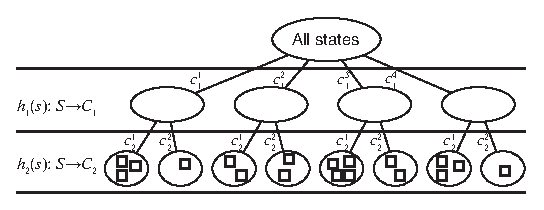
\includegraphics[width=3.2in]{chef/figures/cupa}
  \caption{\cupa state partitioning.  Each level corresponds to a state classification scheme.  Child nodes partition the parent node according to the classification at their level.}
  \label{fig:cupa}
\end{figure}
%
\cupa selects a new state for exploration by performing a random descent in the classification tree, starting from the root.  When reaching a leaf, the strategy takes out a random state from the state set and returns it to the symbolic execution engine for exploration.  By default, all sibling classes on each level have equal probability of being picked, but they can be assigned weights if required.

A \cupa strategy is parameterized by the number $N$ of levels in the tree and a classification function $h_i$ for each level $i=1 \ldots N$.  \chef uses two instantiations of \cupa: one optimized for covering high-level paths (Section~\ref{sec:chef:cupa-paths}) and one for covering the high-level CFG, i.e., statements (Section~\ref{sec:chef:cupa-coverage}).

\subsection{Path-optimized CUPA}
\label{sec:chef:cupa-paths}

The goal of the path-optimized CUPA is to discover high-level paths through the program.  The strategy achieves this by mitigating the bias towards high-level instructions that fork more low-level states than others, such as string operations or native calls.
%
We instantiate a two-level \cupa strategy using the following classes:
\begin{enumerate}
\item The location of the state in the high-level symbolic execution tree.  This is the occurrence of the state's high-level program counter (\hlpc) in the unfolded high-level CFG, referred to as the dynamic \hlpc.  We choose the dynamic \hlpc to give each high-level path reaching the \hlpc the same chance to fork and subsequently diverge.
\item The low-level x86 program counter of the state.  This classification reduces the selection bias of ``hot spots'' of path explosion within a single complex instruction, such as a native function call.
\end{enumerate}

\subsection{Coverage-optimized CUPA}
\label{sec:chef:cupa-coverage}

Coverage-optimized \cupa aims to discover those high-level paths that increase the basic block coverage.
%
Based on a coverage-optimized strategy introduced by the \klee symbolic execution engine~\cite{klee}, we developed a \cupa instance that partitions states according to their minimum distance to branches leading to uncovered code.
%
Alas, dynamic language interpreters do not generally have a static CFG view of the program, so code that has not been covered yet is not accessible to the search strategy.  The high-level CFG of the target program is dynamically discovered along each execution path.  On this CFG, we employ heuristics that (1) identify the instruction opcodes that may branch, and (2)~weigh the state selection toward states that are closer to these potential branching points.

First, \chef identifies the branching opcodes by collecting all high-level instructions that terminate a basic block with an out-degree in the CFG of at least $2$ (i.e., cause branching in the control flow).   We then eliminate the 10\% least frequent opcodes, which correspond to exceptions or other rare control-flow events.
%
Second, \chef identifies the potential branching points as those instructions in the CFG that have a branching opcode (as previously identified) but currently only one successor.
%
Finally, \chef computes for each execution state the distance in the CFG to the closest such potential branching point.

Having computed this information, we instantiate a two-level \cupa strategy with the following classes:
\begin{enumerate}
\item The static \hlpc of the state in the high-level CFG.  On this level, each class is weighted by $\frac{1}{d}$, where $d$ is the distance in the inferred high-level CFG to the closest potential branching point, making states at locations close to a target more likely to be selected.
\item The state itself (so each partition has a single element).  On this level, the states are weighted by their \textit{fork weight}.
\end{enumerate}

Fork weight is computed by counting the number of consecutive forks at the same low-level program counter (i.e., at an input-dependent loop in machine code).  States $1, \ldots, n$ forking from the same path at the same location get weights $p^n, p^{n-1}, \ldots, 1$, where $p < 1$ de-emphasizes states forked earlier ($p = 0.75$ in our implementation).  The last state to fork at a certain location thus gets maximum weight, because alternating the last decision in a loop is often the quickest way to reach different program behavior (e.g., to satisfy a string equality check).

%%% Local Variables: 
%%% mode: latex
%%% eval: (visual-line-mode)
%%% fill-column: 1000000
%%% TeX-master: "main"
%%% End:
